\documentclass[12pt, a4paper]{article}

\usepackage[utf8]{inputenc}
\usepackage[T1]{fontenc}
\usepackage{geometry}
\usepackage{hyperref}
\usepackage{amsmath}
\usepackage{amssymb}
\usepackage{booktabs}
\usepackage[backend=biber, style=authoryear]{biblatex}
\usepackage{tikz}
\usetikzlibrary{positioning,arrows.meta,fit}

\geometry{margin=2.5cm}
\addbibresource{references.bib}

\title{Image Fragment Reconstruction via Adjacency Prediction}
\author{}
\date{\today}

\begin{document}

\maketitle
\tableofcontents
\newpage

% ─────────────────────────────────────────────
\section{Problem Statement}
% ─────────────────────────────────────────────

Let $\mathcal{I} = \{I_1, \dots, I_N\}$ be a set of $N$ source images, each of spatial
resolution $H \times W \times 3$. Each image is divided into a regular $G \times G$ grid
of non-overlapping fragments of size $\frac{H}{G} \times \frac{W}{G} \times 3$, yielding
$G^2$ fragments per image and $M = N \cdot G^2$ fragments in total. In the experimental
setting used here $N = 10$, $H = W = 64$, $G = 4$, giving fragments of size
$16 \times 16 \times 3$ and $M = 160$ fragments per batch.

Let $f_k \in \mathbb{R}^{16 \times 16 \times 3}$ denote fragment $k$, and let
$s(k) \in \{1, \dots, N\}$ be its source image. The fragments from all $N$ images are
pooled into a single unordered collection. The task is:

\begin{quote}
\textit{Given the pooled collection of $M$ fragments with no positional or source
information, assign each fragment to one of $N$ groups such that all fragments assigned
to the same group originate from the same source image.}
\end{quote}

Formally, the goal is to recover a partition $\hat{\mathcal{C}} = \{\hat{C}_1, \dots,
\hat{C}_N\}$ of $\{1, \dots, M\}$ such that for each predicted cluster $\hat{C}_n$ there
exists a source image $I_{s}$ with $s(k) = s$ for all $k \in \hat{C}_n$.

\paragraph{Constraints.}
Two constraints make this non-trivial:

\begin{enumerate}
    \item \textbf{No positional information.} The original grid coordinates of each
          fragment are not provided at inference time. The model may not use absolute
          position as a feature.
    \item \textbf{No labels during training.} The source identity $s(k)$ is never
          provided to the model as a supervisory signal. The model must learn from
          structural properties of the fragments themselves.
\end{enumerate}

\paragraph{Known structure.}
Although labels are withheld, the following quantities are known and may be exploited:
\begin{itemize}
    \item The total number of source images $N = 10$ (so $k = N$ clusters are sought).
    \item Each source image contributes exactly $G^2 = 16$ fragments, so all clusters
          have equal size.
    \item Spatial adjacency within a source image is fully determined by the grid
          structure and can be derived without labels: fragments at grid positions
          $(r, c)$ and $(r', c')$ are adjacent if and only if $|r - r'| + |c - c'| = 1$.
\end{itemize}

The third point is the key observation exploited by the proposed approach (Section~2).

% ─────────────────────────────────────────────
\section{Related Work}
% ─────────────────────────────────────────────

The problem sits at the intersection of self-supervised representation learning and
clustering. We review three families of prior work that informed the approach.

\paragraph{Pretext-task self-supervision.}
The dominant paradigm in self-supervised vision until the rise of contrastive methods
was to define a hand-crafted pretext task whose labels are derivable from the data
itself. \textcite{noroozi2016} solve a jigsaw permutation: given a $3 \times 3$ grid
of fragments shuffled by one of 100 fixed permutations, predict which permutation was
used. The encoder learns features useful for downstream classification. Our adjacency
prediction is a much simpler, binary variant of this idea --- rather than predicting
a discrete permutation index over an exponentially large space, we predict a binary
label per pair. This trades off representational richness for sample efficiency.

\paragraph{Contrastive learning.}
SimCLR \parencite{simclr2020} and MoCo \parencite{moco2020} learn representations by
pulling together augmented views of the same image and pushing apart views of
different images. In the present setting these methods are awkward: there is no
natural positive pair construction, since the natural ``view'' of a fragment is the
fragment itself. One could treat all fragments from one source image as positives
of each other, but this requires the source label that we are explicitly forbidden
to use during training. Adjacency labels, in contrast, are derivable from the grid
structure alone.

\paragraph{Clustering-based self-supervision.}
DeepCluster \parencite{deepcluster2018} alternates between clustering current
embeddings and using cluster assignments as pseudo-labels. SwAV
\parencite{swav2020} extends this with online clustering and equipartitioned cluster
assignments via the Sinkhorn algorithm. Both are conceptually well-suited to this
task, but they introduce significant complexity (alternating training, prototype
maintenance) for what is at heart a small-scale clustering problem with $N = 10$
images. We treat this family as a strong candidate for follow-up work but defer it.

% ─────────────────────────────────────────────
\section{Core Idea}
% ─────────────────────────────────────────────

The central observation is that two fragments cut from the same image and placed next to
each other in the grid share a common boundary — colours bleed over, textures continue,
and objects span tiles. This visual continuity is a strong and reliable signal that does
not require any human annotation to exploit: since the experimenter creates the grid, the
ground-truth adjacency of every fragment pair is known at all times.

The proposed approach uses adjacency prediction as a \textbf{pretext task}
\parencite{noroozi2016}. The model is trained to solve a surrogate problem — predicting
whether two fragments are spatially adjacent — and in doing so is forced to learn visual
representations that capture source identity as a side effect. At inference time the
pretext objective is discarded and the learned representations are used for clustering.

This is self-supervised throughout: no labels beyond those derivable from the grid
structure are ever used.

% ─────────────────────────────────────────────
\section{Architecture: Siamese Network}
% ─────────────────────────────────────────────

The model is a Siamese network: a shared encoder is applied to each of two input
fragments, and a comparison head turns the two embeddings into a binary
prediction (Figure~\ref{fig:architecture}). When the multi-task loss is enabled,
a second comparison head with the same structure is added for same-image
prediction.

\begin{figure}[h]
\centering
% Standalone TikZ figure: schematic of the Siamese fragment-pair model.
%
% Include in another document with:
%     % Standalone TikZ figure: schematic of the Siamese fragment-pair model.
%
% Include in another document with:
%     % Standalone TikZ figure: schematic of the Siamese fragment-pair model.
%
% Include in another document with:
%     \input{fig_architecture.tex}
%
% Requires the host document to load \usepackage{tikz} and the libraries
% positioning, arrows.meta, fit. Compile fig_architecture_standalone.tex
% to preview.

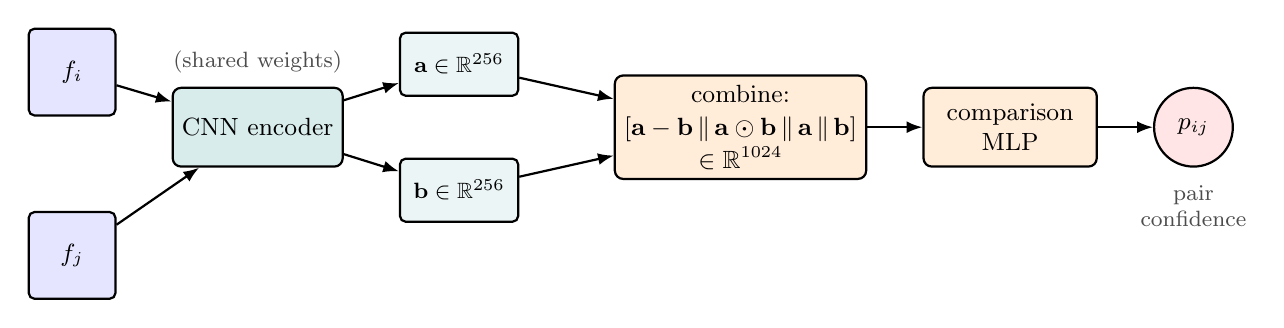
\begin{tikzpicture}[
    node distance = 6mm and 7mm,
    frag/.style   = {draw, thick, rounded corners=2pt, minimum width=11mm,
                     minimum height=11mm, fill=blue!10, font=\small},
    enc/.style    = {draw, thick, rounded corners=3pt, minimum width=18mm,
                     minimum height=10mm, fill=teal!15, font=\small},
    emb/.style    = {draw, thick, rounded corners=2pt, minimum width=15mm,
                     minimum height=8mm, fill=teal!8, font=\footnotesize},
    head/.style   = {draw, thick, rounded corners=3pt, minimum width=22mm,
                     minimum height=10mm, fill=orange!15, font=\small},
    output/.style = {draw, thick, circle, minimum size=10mm,
                     fill=red!10, font=\small, inner sep=0pt},
    arr/.style    = {-{Latex[length=2mm]}, thick},
    note/.style   = {font=\footnotesize, color=black!70},
]

% --- inputs: two fragments ---
\node[frag] (f1) {$f_i$};
\node[frag, below=12mm of f1] (f2) {$f_j$};

% --- shared encoder (drawn once, with arrows from both fragments) ---
\node[enc, right=of f1, yshift=-7mm] (enc) {CNN encoder};
\node[note, above=0.5mm of enc] {(shared weights)};

% --- per-fragment embeddings ---
\node[emb, right=of enc, yshift=8mm]  (e1) {$\mathbf{a} \in \mathbb{R}^{256}$};
\node[emb, right=of enc, yshift=-8mm] (e2) {$\mathbf{b} \in \mathbb{R}^{256}$};

% --- combination block ---
\node[head, right=12mm of e1, yshift=-8mm,
      align=center] (combine)
      {combine:\\[1pt] $[\mathbf{a}-\mathbf{b}\,\|\,\mathbf{a}\odot\mathbf{b}\,\|\,\mathbf{a}\,\|\,\mathbf{b}]$\\[1pt]
       $\in \mathbb{R}^{1024}$};

% --- single comparison head ---
\node[head, right=of combine, align=center] (head)
    {comparison\\MLP};

% --- output ---
\node[output, right=of head] (p) {$p_{ij}$};

% --- arrows ---
\draw[arr] (f1) -- (enc);
\draw[arr] (f2) -- (enc);
\draw[arr] (enc) -- (e1);
\draw[arr] (enc) -- (e2);
\draw[arr] (e1) -- (combine);
\draw[arr] (e2) -- (combine);
\draw[arr] (combine) -- (head);
\draw[arr] (head) -- (p);

% --- annotation under output ---
\node[note, below=1mm of p, align=center]
    {pair\\confidence};

\end{tikzpicture}

%
% Requires the host document to load \usepackage{tikz} and the libraries
% positioning, arrows.meta, fit. Compile fig_architecture_standalone.tex
% to preview.

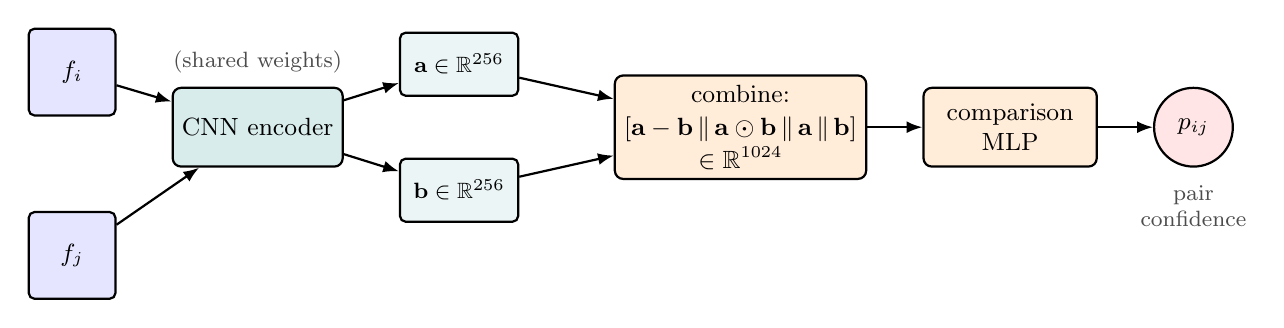
\begin{tikzpicture}[
    node distance = 6mm and 7mm,
    frag/.style   = {draw, thick, rounded corners=2pt, minimum width=11mm,
                     minimum height=11mm, fill=blue!10, font=\small},
    enc/.style    = {draw, thick, rounded corners=3pt, minimum width=18mm,
                     minimum height=10mm, fill=teal!15, font=\small},
    emb/.style    = {draw, thick, rounded corners=2pt, minimum width=15mm,
                     minimum height=8mm, fill=teal!8, font=\footnotesize},
    head/.style   = {draw, thick, rounded corners=3pt, minimum width=22mm,
                     minimum height=10mm, fill=orange!15, font=\small},
    output/.style = {draw, thick, circle, minimum size=10mm,
                     fill=red!10, font=\small, inner sep=0pt},
    arr/.style    = {-{Latex[length=2mm]}, thick},
    note/.style   = {font=\footnotesize, color=black!70},
]

% --- inputs: two fragments ---
\node[frag] (f1) {$f_i$};
\node[frag, below=12mm of f1] (f2) {$f_j$};

% --- shared encoder (drawn once, with arrows from both fragments) ---
\node[enc, right=of f1, yshift=-7mm] (enc) {CNN encoder};
\node[note, above=0.5mm of enc] {(shared weights)};

% --- per-fragment embeddings ---
\node[emb, right=of enc, yshift=8mm]  (e1) {$\mathbf{a} \in \mathbb{R}^{256}$};
\node[emb, right=of enc, yshift=-8mm] (e2) {$\mathbf{b} \in \mathbb{R}^{256}$};

% --- combination block ---
\node[head, right=12mm of e1, yshift=-8mm,
      align=center] (combine)
      {combine:\\[1pt] $[\mathbf{a}-\mathbf{b}\,\|\,\mathbf{a}\odot\mathbf{b}\,\|\,\mathbf{a}\,\|\,\mathbf{b}]$\\[1pt]
       $\in \mathbb{R}^{1024}$};

% --- single comparison head ---
\node[head, right=of combine, align=center] (head)
    {comparison\\MLP};

% --- output ---
\node[output, right=of head] (p) {$p_{ij}$};

% --- arrows ---
\draw[arr] (f1) -- (enc);
\draw[arr] (f2) -- (enc);
\draw[arr] (enc) -- (e1);
\draw[arr] (enc) -- (e2);
\draw[arr] (e1) -- (combine);
\draw[arr] (e2) -- (combine);
\draw[arr] (combine) -- (head);
\draw[arr] (head) -- (p);

% --- annotation under output ---
\node[note, below=1mm of p, align=center]
    {pair\\confidence};

\end{tikzpicture}

%
% Requires the host document to load \usepackage{tikz} and the libraries
% positioning, arrows.meta, fit. Compile fig_architecture_standalone.tex
% to preview.

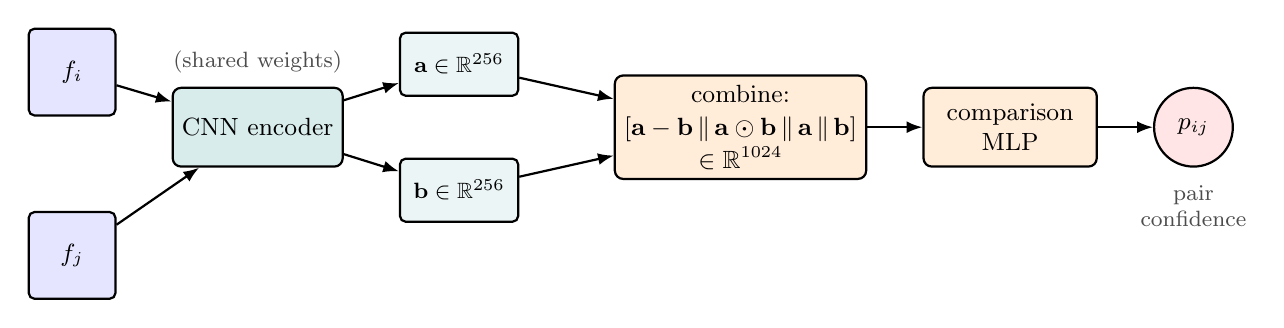
\begin{tikzpicture}[
    node distance = 6mm and 7mm,
    frag/.style   = {draw, thick, rounded corners=2pt, minimum width=11mm,
                     minimum height=11mm, fill=blue!10, font=\small},
    enc/.style    = {draw, thick, rounded corners=3pt, minimum width=18mm,
                     minimum height=10mm, fill=teal!15, font=\small},
    emb/.style    = {draw, thick, rounded corners=2pt, minimum width=15mm,
                     minimum height=8mm, fill=teal!8, font=\footnotesize},
    head/.style   = {draw, thick, rounded corners=3pt, minimum width=22mm,
                     minimum height=10mm, fill=orange!15, font=\small},
    output/.style = {draw, thick, circle, minimum size=10mm,
                     fill=red!10, font=\small, inner sep=0pt},
    arr/.style    = {-{Latex[length=2mm]}, thick},
    note/.style   = {font=\footnotesize, color=black!70},
]

% --- inputs: two fragments ---
\node[frag] (f1) {$f_i$};
\node[frag, below=12mm of f1] (f2) {$f_j$};

% --- shared encoder (drawn once, with arrows from both fragments) ---
\node[enc, right=of f1, yshift=-7mm] (enc) {CNN encoder};
\node[note, above=0.5mm of enc] {(shared weights)};

% --- per-fragment embeddings ---
\node[emb, right=of enc, yshift=8mm]  (e1) {$\mathbf{a} \in \mathbb{R}^{256}$};
\node[emb, right=of enc, yshift=-8mm] (e2) {$\mathbf{b} \in \mathbb{R}^{256}$};

% --- combination block ---
\node[head, right=12mm of e1, yshift=-8mm,
      align=center] (combine)
      {combine:\\[1pt] $[\mathbf{a}-\mathbf{b}\,\|\,\mathbf{a}\odot\mathbf{b}\,\|\,\mathbf{a}\,\|\,\mathbf{b}]$\\[1pt]
       $\in \mathbb{R}^{1024}$};

% --- single comparison head ---
\node[head, right=of combine, align=center] (head)
    {comparison\\MLP};

% --- output ---
\node[output, right=of head] (p) {$p_{ij}$};

% --- arrows ---
\draw[arr] (f1) -- (enc);
\draw[arr] (f2) -- (enc);
\draw[arr] (enc) -- (e1);
\draw[arr] (enc) -- (e2);
\draw[arr] (e1) -- (combine);
\draw[arr] (e2) -- (combine);
\draw[arr] (combine) -- (head);
\draw[arr] (head) -- (p);

% --- annotation under output ---
\node[note, below=1mm of p, align=center]
    {pair\\confidence};

\end{tikzpicture}

\caption{Schematic of the model. The CNN encoder is applied with shared weights
to each of two input fragments; its $256$-dimensional embeddings are combined into a
single $1024$-dimensional vector via concatenation of difference, element-wise
product, and the two embeddings themselves; this vector is fed to one or two
comparison heads (adjacency, same-image) that produce binary predictions.}
\label{fig:architecture}
\end{figure}

The components are:

\paragraph{Shared CNN encoder.}
A single convolutional neural network maps each 16$\times$16$\times$3 fragment to a
256-dimensional embedding vector. The architecture is three convolutional blocks
(Conv--BatchNorm--ReLU), with max-pooling after blocks two and three, reducing the
spatial dimensions from $16\times16$ to $4\times4$. The flattened $4\times4\times128$
feature map is projected to a 256-dimensional embedding via a linear layer followed by
ReLU and dropout ($p=0.3$).

The encoder is \textbf{shared} — the same weights are used for both fragments in a pair.
This is the defining property of a Siamese network \parencite{siamese1994}: weight
sharing ensures that the comparison is symmetric and that the encoder learns a universal
fragment representation rather than one tuned to a specific input slot.

\paragraph{Comparison head (MLP).}
A small multi-layer perceptron takes as input a 1024-dimensional vector formed by
concatenating four interaction terms between the two embeddings $\mathbf{a} =
\text{CNN}(f_i)$ and $\mathbf{b} = \text{CNN}(f_j)$:

\[
\mathbf{z}_{ij} = \bigl[\mathbf{a} - \mathbf{b} \;\|\; \mathbf{a} \odot \mathbf{b} \;\|\; \mathbf{a} \;\|\; \mathbf{b}\bigr] \in \mathbb{R}^{1024}
\]

The difference $\mathbf{a} - \mathbf{b}$ captures asymmetric discrepancies; the
element-wise product $\mathbf{a} \odot \mathbf{b}$ captures feature co-activation; and
including both raw embeddings preserves their individual information. The MLP maps
$\mathbf{z}_{ij}$ through a hidden layer of size 128 (ReLU) to a single scalar in
$[0, 1]$:

\[
p_{ij} = \sigma\!\bigl(W_2\,\text{ReLU}(W_1\,\mathbf{z}_{ij} + b_1) + b_2\bigr)
\]

% ─────────────────────────────────────────────
\section{Training}
% ─────────────────────────────────────────────

\subsection{Constructing Training Labels}

From a sample of 10 images cut into a 4$\times$4 grid, each fragment has at most 4
adjacent neighbours (fewer at corners and edges). For a sample of 160 fragments the
total number of pairs is:

\[
\binom{160}{2} = 12{,}720
\]

Each pair receives a binary label: $y_{ij} = 1$ if the two fragments are adjacent within
the same image, $y_{ij} = 0$ otherwise. This label is derived entirely from the known
grid positions and requires no human annotation
(Figure~\ref{fig:grid-labels}).

\begin{figure}[h]
\centering
% Standalone TikZ figure: a 4x4 grid of fragments, with adjacency edges
% highlighted, used to illustrate how training labels are constructed.
%
% Include in another document with:
%     % Standalone TikZ figure: a 4x4 grid of fragments, with adjacency edges
% highlighted, used to illustrate how training labels are constructed.
%
% Include in another document with:
%     % Standalone TikZ figure: a 4x4 grid of fragments, with adjacency edges
% highlighted, used to illustrate how training labels are constructed.
%
% Include in another document with:
%     \input{fig_grid_labels.tex}
%
% Requires the host document to load \usepackage{tikz}. Compile
% fig_grid_labels_standalone.tex to preview.

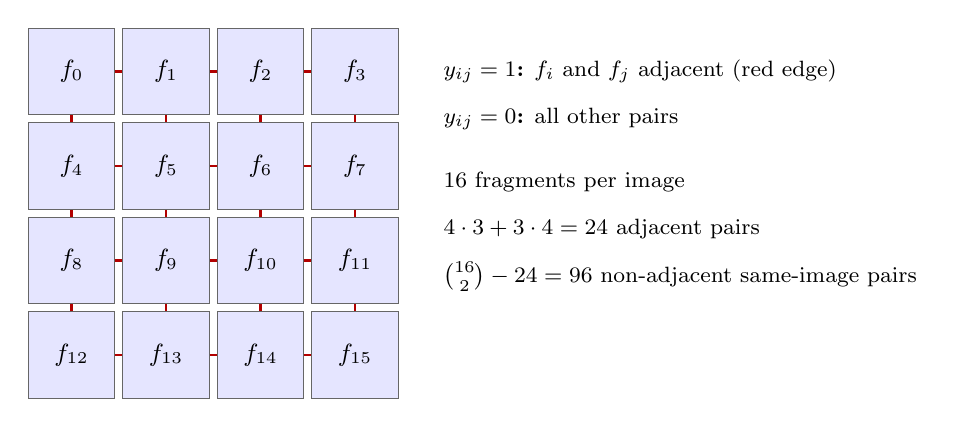
\begin{tikzpicture}[
    cell/.style    = {draw=black!60, fill=blue!10, minimum size=11mm,
                      inner sep=0pt, font=\small},
    edge/.style    = {color=red!70!black, line width=1pt},
]

% --- 4x4 grid of cells ---
\foreach \r in {0,1,2,3}{
    \foreach \c in {0,1,2,3}{
        \pgfmathtruncatemacro{\idx}{\r*4 + \c}
        \node[cell] (n\r\c) at (\c*1.2, -\r*1.2) {$f_{\idx}$};
    }
}

% --- horizontal adjacency edges ---
\foreach \r in {0,1,2,3}{
    \foreach \c in {0,1,2}{
        \pgfmathtruncatemacro{\cnext}{\c+1}
        \draw[edge] (n\r\c) -- (n\r\cnext);
    }
}

% --- vertical adjacency edges ---
\foreach \c in {0,1,2,3}{
    \foreach \r in {0,1,2}{
        \pgfmathtruncatemacro{\rnext}{\r+1}
        \draw[edge] (n\r\c) -- (n\rnext\c);
    }
}

% --- legend ---
\node[anchor=west, font=\footnotesize] at (4.6, 0)
    {\textbf{$y_{ij} = 1$:} $f_i$ and $f_j$ adjacent (red edge)};
\node[anchor=west, font=\footnotesize] at (4.6, -0.6)
    {\textbf{$y_{ij} = 0$:} all other pairs};
\node[anchor=west, font=\footnotesize] at (4.6, -1.4)
    {16 fragments per image};
\node[anchor=west, font=\footnotesize] at (4.6, -2.0)
    {$4 \cdot 3 + 3 \cdot 4 = 24$ adjacent pairs};
\node[anchor=west, font=\footnotesize] at (4.6, -2.6)
    {$\binom{16}{2} - 24 = 96$ non-adjacent same-image pairs};

\end{tikzpicture}

%
% Requires the host document to load \usepackage{tikz}. Compile
% fig_grid_labels_standalone.tex to preview.

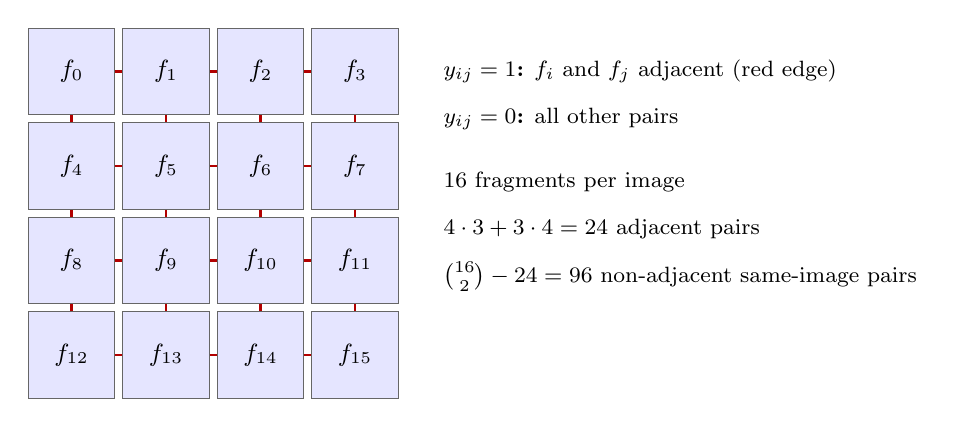
\begin{tikzpicture}[
    cell/.style    = {draw=black!60, fill=blue!10, minimum size=11mm,
                      inner sep=0pt, font=\small},
    edge/.style    = {color=red!70!black, line width=1pt},
]

% --- 4x4 grid of cells ---
\foreach \r in {0,1,2,3}{
    \foreach \c in {0,1,2,3}{
        \pgfmathtruncatemacro{\idx}{\r*4 + \c}
        \node[cell] (n\r\c) at (\c*1.2, -\r*1.2) {$f_{\idx}$};
    }
}

% --- horizontal adjacency edges ---
\foreach \r in {0,1,2,3}{
    \foreach \c in {0,1,2}{
        \pgfmathtruncatemacro{\cnext}{\c+1}
        \draw[edge] (n\r\c) -- (n\r\cnext);
    }
}

% --- vertical adjacency edges ---
\foreach \c in {0,1,2,3}{
    \foreach \r in {0,1,2}{
        \pgfmathtruncatemacro{\rnext}{\r+1}
        \draw[edge] (n\r\c) -- (n\rnext\c);
    }
}

% --- legend ---
\node[anchor=west, font=\footnotesize] at (4.6, 0)
    {\textbf{$y_{ij} = 1$:} $f_i$ and $f_j$ adjacent (red edge)};
\node[anchor=west, font=\footnotesize] at (4.6, -0.6)
    {\textbf{$y_{ij} = 0$:} all other pairs};
\node[anchor=west, font=\footnotesize] at (4.6, -1.4)
    {16 fragments per image};
\node[anchor=west, font=\footnotesize] at (4.6, -2.0)
    {$4 \cdot 3 + 3 \cdot 4 = 24$ adjacent pairs};
\node[anchor=west, font=\footnotesize] at (4.6, -2.6)
    {$\binom{16}{2} - 24 = 96$ non-adjacent same-image pairs};

\end{tikzpicture}

%
% Requires the host document to load \usepackage{tikz}. Compile
% fig_grid_labels_standalone.tex to preview.

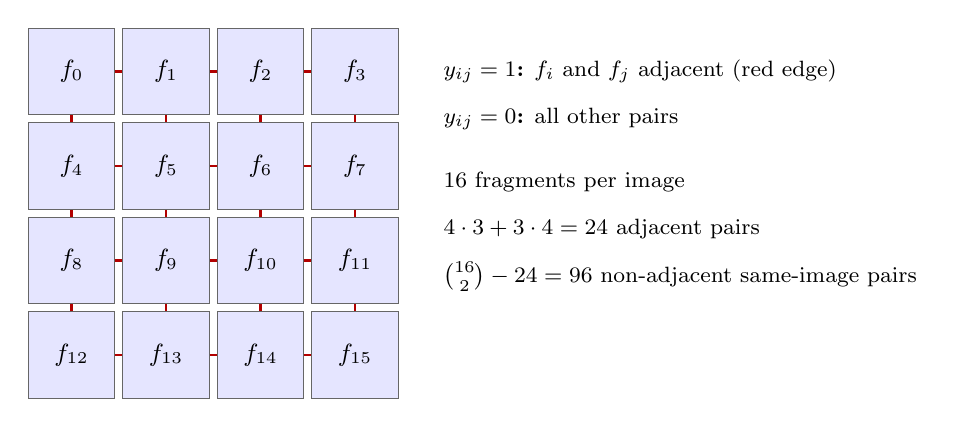
\begin{tikzpicture}[
    cell/.style    = {draw=black!60, fill=blue!10, minimum size=11mm,
                      inner sep=0pt, font=\small},
    edge/.style    = {color=red!70!black, line width=1pt},
]

% --- 4x4 grid of cells ---
\foreach \r in {0,1,2,3}{
    \foreach \c in {0,1,2,3}{
        \pgfmathtruncatemacro{\idx}{\r*4 + \c}
        \node[cell] (n\r\c) at (\c*1.2, -\r*1.2) {$f_{\idx}$};
    }
}

% --- horizontal adjacency edges ---
\foreach \r in {0,1,2,3}{
    \foreach \c in {0,1,2}{
        \pgfmathtruncatemacro{\cnext}{\c+1}
        \draw[edge] (n\r\c) -- (n\r\cnext);
    }
}

% --- vertical adjacency edges ---
\foreach \c in {0,1,2,3}{
    \foreach \r in {0,1,2}{
        \pgfmathtruncatemacro{\rnext}{\r+1}
        \draw[edge] (n\r\c) -- (n\rnext\c);
    }
}

% --- legend ---
\node[anchor=west, font=\footnotesize] at (4.6, 0)
    {\textbf{$y_{ij} = 1$:} $f_i$ and $f_j$ adjacent (red edge)};
\node[anchor=west, font=\footnotesize] at (4.6, -0.6)
    {\textbf{$y_{ij} = 0$:} all other pairs};
\node[anchor=west, font=\footnotesize] at (4.6, -1.4)
    {16 fragments per image};
\node[anchor=west, font=\footnotesize] at (4.6, -2.0)
    {$4 \cdot 3 + 3 \cdot 4 = 24$ adjacent pairs};
\node[anchor=west, font=\footnotesize] at (4.6, -2.6)
    {$\binom{16}{2} - 24 = 96$ non-adjacent same-image pairs};

\end{tikzpicture}

\caption{Adjacency labelling within a single source image. Each of the 16
fragments is connected by a red edge to each of its grid neighbours. The
24 highlighted edges are the positive pairs ($y_{ij} = 1$); all other pairs
within the image (96 of them) and across images are negative ($y_{ij} = 0$).}
\label{fig:grid-labels}
\end{figure}

\subsection{Loss Function}

Binary cross-entropy is the natural loss for a binary prediction task:

\[
\mathcal{L}_{\text{BCE}} = -\frac{1}{N}\sum_{(i,j)} \Bigl[ y_{ij} \log p_{ij} + (1 - y_{ij}) \log(1 - p_{ij}) \Bigr]
\]

Positive (adjacent) pairs are far rarer than negative pairs in this configuration.
With 10 source images on a $4 \times 4$ grid, each image contributes
$4 \cdot 3 + 3 \cdot 4 = 24$ adjacent pairs, giving $n_{+} = 240$ positives in
total. The remaining pairs are negatives: $n_{-} = \binom{160}{2} - 240 = 12{,}480$.
The ratio $n_{-}/n_{+} = 52$ is therefore a constant determined by the grid
geometry, not a per-batch quantity. Vanilla BCE on this data is dominated by the
negative class: the gradient is overwhelmingly driven by the loss on non-adjacent
pairs, and the model has little incentive to identify the few adjacent ones. The
standard remedy is to upweight the rare class. Since only the ratio of the two
class weights matters, we parameterise the loss with a single \emph{tilt}
parameter $\beta \geq 1$:
\[
\mathcal{L}_{\text{WBCE}}(\beta) = -\frac{1}{N}\sum_{(i,j)}
    \Bigl[\, \beta \cdot \tfrac{n_{-}}{n_{+}}\, y_{ij} \log p_{ij}
       + (1 - y_{ij}) \log(1 - p_{ij}) \,\Bigr].
\]

The textbook value is $\beta = 1$, the class-balanced loss: it equalises the
total gradient contribution of the two classes, treating a single positive as
worth 52 negatives. Setting $\beta > 1$ over-weights positives beyond this
point --- a positive mistake is now \emph{more} costly than the natural class
ratio implies. For our downstream task this is desirable, and we expect the
optimum to lie at a moderate-to-aggressive tilt.

\paragraph{Why we lean toward a moderate-to-aggressive tilt.}
The downstream task is graph clustering, not per-edge classification. False
negatives directly weaken intra-cluster connectivity, while false positives are
only harmful when they connect fragments from \emph{different} source images ---
a case the model rarely produces because cross-image fragments are visually
dissimilar. Same-image false positives, the more common kind, actually reinforce
the connectivity spectral clustering relies on. The error costs are therefore
asymmetric in favour of recall, and we expect the optimal $\beta$ to lie above
the class-balanced point.

\subsection{Computational Cost}

The CNN encoder runs once per fragment (160 forward passes per sample). All pairwise
embeddings are then combined using tensor operations, and the lightweight MLP processes
all 12,720 pairs. Since the expensive step (the CNN) runs only 160 times, the
computational overhead is manageable.

% ─────────────────────────────────────────────
\section{From Pretext Task to Clustering}
% ─────────────────────────────────────────────

After training, the model produces a value $p_{ij} \in [0, 1]$ for every pair of
fragments. We do not interpret this as a calibrated probability --- the model is
trained on a binary cross-entropy objective but its outputs are not guaranteed to
be calibrated to true frequencies. We use $p_{ij}$ instead as a confidence score:
the higher the value, the more confident the model is that fragments $i$ and $j$
are adjacent. These scores define a \textbf{fully connected weighted graph} over
the 160 fragments, where edge weight $w_{ij} = p_{ij}$ reflects the model's
confidence that the two fragments are adjacent --- and by extension, that they
originate from the same image (Figure~\ref{fig:similarity-graph}).

\begin{figure}[h]
\centering
% Standalone TikZ figure: predicted similarity graph over fragments.
%
% This file contains only the \begin{tikzpicture} ... \end{tikzpicture} block,
% so it can be \input{} into any host document that loads tikz. To preview as
% a standalone PDF, compile fig_similarity_graph_standalone.tex.

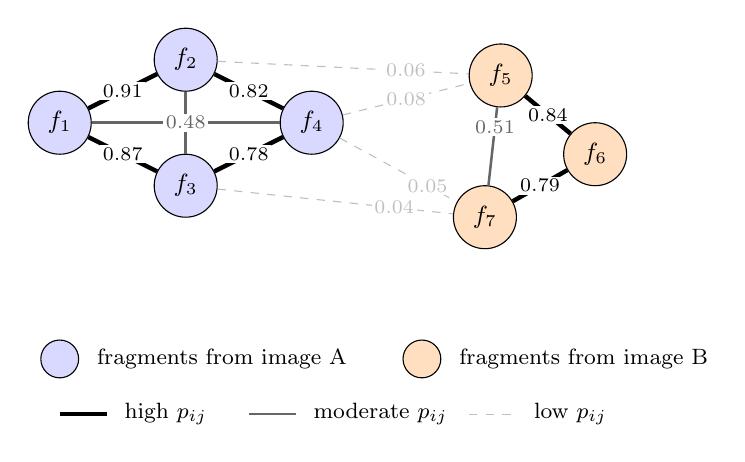
\begin{tikzpicture}[
    node/.style    = {circle, draw, minimum size=8mm, inner sep=0pt, font=\small},
    src1/.style    = {node, fill=blue!15},
    src2/.style    = {node, fill=orange!25},
    edge/.style    = {-, line width=0.6pt},
    strong/.style  = {edge, color=black, line width=1.6pt},
    medium/.style  = {edge, color=black!60, line width=0.9pt},
    weak/.style    = {edge, color=black!25, line width=0.4pt, dashed},
    weight/.style  = {font=\scriptsize, fill=white, inner sep=1pt},
]

% --- nodes: 4 fragments from image A (blue), 3 from image B (orange) ---
\node[src1] (a1) at (0, 2)         {$f_1$};
\node[src1] (a2) at (1.6, 2.8)     {$f_2$};
\node[src1] (a3) at (1.6, 1.2)     {$f_3$};
\node[src1] (a4) at (3.2, 2)       {$f_4$};

\node[src2] (b1) at (5.6, 2.6)     {$f_5$};
\node[src2] (b2) at (6.8, 1.6)     {$f_6$};
\node[src2] (b3) at (5.4, 0.8)     {$f_7$};

% --- intra-A edges (high probability, drawn strong) ---
\draw[strong] (a1) -- (a2) node[weight, midway] {$0.91$};
\draw[strong] (a1) -- (a3) node[weight, midway] {$0.87$};
\draw[strong] (a2) -- (a4) node[weight, midway] {$0.82$};
\draw[strong] (a3) -- (a4) node[weight, midway] {$0.78$};
\draw[medium] (a1) -- (a4) node[weight, midway] {$0.55$};
\draw[medium] (a2) -- (a3) node[weight, midway] {$0.48$};

% --- intra-B edges ---
\draw[strong] (b1) -- (b2) node[weight, midway] {$0.84$};
\draw[strong] (b2) -- (b3) node[weight, midway] {$0.79$};
\draw[medium] (b1) -- (b3) node[weight, near start] {$0.51$};

% --- cross edges (low probability, weak/dashed) ---
\draw[weak] (a4) -- (b1) node[weight, midway] {$0.08$};
\draw[weak] (a4) -- (b3) node[weight, near end] {$0.05$};
\draw[weak] (a2) -- (b1) node[weight, near end] {$0.06$};
\draw[weak] (a3) -- (b3) node[weight, near end] {$0.04$};

% --- legend ---
\begin{scope}[shift={(0, -1.0)}]
    \node[src1, scale=0.6] (lg1) at (0, 0) {};
    \node[anchor=west, font=\footnotesize] at (0.35, 0) {fragments from image A};

    \node[src2, scale=0.6] (lg2) at (4.6, 0) {};
    \node[anchor=west, font=\footnotesize] at (4.95, 0) {fragments from image B};
\end{scope}

\begin{scope}[shift={(0, -1.7)}]
    \draw[strong] (0, 0) -- (0.6, 0);
    \node[anchor=west, font=\footnotesize] at (0.7, 0) {high $p_{ij}$};

    \draw[medium] (2.4, 0) -- (3.0, 0);
    \node[anchor=west, font=\footnotesize] at (3.1, 0) {moderate $p_{ij}$};

    \draw[weak] (5.2, 0) -- (5.8, 0);
    \node[anchor=west, font=\footnotesize] at (5.9, 0) {low $p_{ij}$};
\end{scope}

\end{tikzpicture}

\caption{Schematic of the predicted similarity graph. Each node is a fragment; edge
weight $p_{ij}$ is the model's confidence that the two fragments are adjacent.
Edges within a true source image (here, two illustrative source images shown in blue
and orange) tend to receive high weight; cross-image edges receive low weight.
Spectral clustering recovers the source-image partition by finding the cut that
separates the densely-connected sub-graphs.}
\label{fig:similarity-graph}
\end{figure}

\paragraph{Balanced spectral clustering.}
\textbf{Spectral clustering} is the natural choice for a weighted graph. Given the
$160 \times 160$ similarity matrix $W$ with $w_{ij} = p_{ij}$, define the diagonal
degree matrix $D$ with $D_{ii} = \sum_j w_{ij}$ and the symmetric normalised graph
Laplacian
\[
L_{\text{sym}} = I - D^{-1/2} W D^{-1/2}.
\]
The spectral embedding stacks the $k$ leading eigenvectors of $L_{\text{sym}}$ into a
$160 \times k$ matrix; in the eigenspace, fragments belonging to densely-connected
sub-graphs lie close together. The standard pipeline then runs $k$-means on this
embedding to obtain hard cluster assignments.

Plain $k$-means ignores the fact that each true cluster contains exactly $G^2 = 16$
fragments and can produce groups of very unequal size. We enforce balance by replacing
the $k$-means step with a balanced assignment: build a $160 \times (k \cdot G^2)$ cost
matrix in which each cluster appears $G^2$ times, and solve the resulting linear
assignment problem with the Hungarian algorithm\footnote{Implemented using
\texttt{sklearn.manifold.SpectralEmbedding} for the eigendecomposition and
\texttt{scipy.optimize.linear\_sum\_assignment} for the assignment.}. Cluster
centroids are then re-estimated and the assignment iterated until convergence
(typically a handful of iterations). The result is a partition of the 160 fragments
into 10 clusters of size 16, by construction.

% ─────────────────────────────────────────────
\section{Evaluation Metric for the Clustering Task}

The pretext task (adjacency prediction) and the downstream task (clustering of
fragments by source image) are evaluated with different metrics. Adjacency
prediction is evaluated with the threshold-free metrics AUROC and AUPRC (described
below in the multi-batch averaging paragraph); the downstream clustering is
evaluated with the \textbf{Adjusted Rand Index (ARI)}. We focus on the clustering
metric here since it is the headline number for this work.

\paragraph{Definition.}
Let $\mathcal{C} = \{C_1, \dots, C_N\}$ be the true partition of the fragments
into $N = 10$ source-image groups, and $\hat{\mathcal{C}} = \{\hat{C}_1, \dots,
\hat{C}_N\}$ the partition predicted by the model. For each pair of fragments, look
at whether the two are in the same true group and whether they are in the same
predicted cluster:

\begin{itemize}
    \item $a$ = number of pairs in the same true group \emph{and} the same predicted cluster
    \item $b$ = number of pairs in different true groups \emph{and} different predicted clusters
    \item $c$ = number of pairs in the same true group but different predicted clusters
    \item $d$ = number of pairs in different true groups but the same predicted cluster
\end{itemize}

The (unadjusted) Rand Index is the agreement rate $\text{RI} = (a + b) / (a + b + c + d)$.
The Adjusted Rand Index normalises this against the expected RI under random labellings
of fixed cluster sizes:
\[
\text{ARI} = \frac{\text{RI} - \mathbb{E}[\text{RI}]}{\max(\text{RI}) - \mathbb{E}[\text{RI}]}.
\]
A random clustering scores $\text{ARI} = 0$, a perfect one scores $\text{ARI} = 1$,
and a clustering worse than random can score below zero.

\paragraph{Why ARI rather than purity.}
ARI is preferred over simpler metrics like purity because purity only looks at the
dominant true class in each predicted cluster and ignores how the remaining errors
are distributed.

\begin{quote}\small
\textbf{Example.} Suppose two predicted clusters each have $60\%$ fragments
from image~A. The first additionally has $40\%$ from image~B; the second has $20\%$
from B and $20\%$ from C. Both clusters score the same purity (0.60), even though
the second is visibly more disordered. ARI distinguishes the two cases because it
counts pair-level agreements rather than looking only at the plurality label.
\end{quote}

\textbf{NMI (Normalised Mutual Information)} is reported alongside ARI as a
complementary metric. It measures how much information the predicted clusters share
with the true groupings, normalised to $[0, 1]$.

\paragraph{Multi-batch averaging.}
Each evaluation step samples a fresh batch of 10 source images from the validation
generator. Because individual batches vary substantially in difficulty (some draws of
10 ImageNet classes are visually well-separated, others contain near-duplicates), a
single-batch ARI estimate has high variance. We average each metric over
$n_{\text{eval}} = 20$ fresh validation batches per evaluation step. This stabilises
the training curves and, crucially, the early-stopping decision and the
checkpoint-selection criterion, which would otherwise be biased toward lucky batches.

% ─────────────────────────────────────────────
\section{Experimental Setup}
% ─────────────────────────────────────────────

\paragraph{Data.}
ImageNet-64 \parencite{imagenet64}: a downsampled version of the ImageNet-1k
classification dataset in which every image has been resized to $64 \times 64$
pixels. The dataset is split into a training partition and a test partition; we draw
the model's training images from the former and the validation images from the
latter. Each training step samples 10 random images on the fly and produces a fresh
batch of 160 fragments; the data generator is therefore effectively infinite. The
augmentation pipeline (rotation up to $\pm 20^\circ$, horizontal/vertical shift up
to 10\%, channel shift 0.2) is applied to the full image \emph{before} fragmentation
and is provided by the dataset's data generator (\texttt{data.py}); it is not
modified.

\paragraph{Hardware.}
All training and evaluation reported in this document was performed on a MacBook Air
(Apple M-series CPU). PyTorch is configured to fall back to CPU; no GPU is required.
A full training run completes in approximately 20--25 minutes on this hardware.

\paragraph{Reproducibility.}
\begin{itemize}
    \item Each run writes its full configuration, training log, and best checkpoint
          into \texttt{runs/\{run\_name\}/}, and appends a one-line summary to
          \texttt{results.jsonl}. The configuration is therefore self-contained and
          re-runnable.
    \item Random seeds are fixed for the clustering routines\footnote{%
          \texttt{random\_state = 42} in
          \texttt{sklearn.cluster.SpectralClustering},
          \texttt{sklearn.cluster.KMeans}, and
          \texttt{sklearn.manifold.SpectralEmbedding}.}.
          The PyTorch random seed is \emph{not} currently fixed, so model
          initialisation and the order of training batches vary between runs; this
          is by design --- repeated runs with different seeds give a sense of the
          variance in final ARI.
    \item Hyperparameters and run metadata are versioned in \texttt{config.yaml}.
\end{itemize}

\paragraph{Hyperparameters.}
The complete list of hyperparameters is maintained in \texttt{config.yaml} and may
still change in the course of further ablations. The current values are documented
there; this section will be replaced with a final hyperparameter table once the
study is complete.

% ─────────────────────────────────────────────
\section{Results}
% ─────────────────────────────────────────────

\subsection{Effect of the loss tilt parameter $\beta$}

We evaluated three settings of the WBCE tilt parameter --- $\beta \in
\{0.019, 0.3, 1.0\}$, corresponding respectively to plain unweighted BCE
($\beta \cdot 52 = 1$), a mild upweighting of positives, and the textbook
class-balanced weighting ($w_{+} = 52$). All three runs use the same
architecture, balanced spectral clustering, and validation averaging over
$n_{\text{eval}} = 20$ fresh batches.

\begin{center}
\begin{tabular}{lccc}
\toprule
\textbf{Run} & \textbf{$\beta$} & \textbf{Best ARI} & \textbf{AUROC / AUPRC} \\
\midrule
\texttt{plain\_bce}     & $0.019$ & $0.535$ & $0.969 \,/\, 0.432$ \\
\texttt{wbce\_beta\_03} & $0.3$   & $0.523$ & $0.973 \,/\, 0.435$ \\
\texttt{wbce\_beta\_1}  & $1.0$   & $0.462$ & $0.969 \,/\, 0.405$ \\
\bottomrule
\end{tabular}
\end{center}

\paragraph{Discussion.}
The choice of $\beta$ has an essentially negligible effect on AUROC: across two
orders of magnitude in $\beta$, ranking quality on the adjacency task varies by
less than a percentage point ($0.969$--$0.973$). What changes with $\beta$ is
the model's \emph{calibration} --- its tendency to push probabilities high or
low overall --- not the order in which it ranks pairs. Because spectral
clustering operates on the raw probabilities as edge weights, both ranking and
calibration matter for ARI, which is why ARI varies a little more than
AUROC ($0.46$--$0.54$).

The variation we observe in ARI is, however, on the same order as the
run-to-run noise we estimated by repeating $\beta = 0.3$ and $\beta = 1$ with
different random seeds: between repeated runs of the same configuration the
ARI changed by up to $\sim 0.05$, comparable to the differences between
configurations. The cleanest reading of the data is that \emph{within the
range tested, $\beta$ is a second-order knob}. Plain BCE performs at least as
well as any weighted variant we tried.

This contradicts the prior expectation expressed earlier in the document
that an aggressive tilt $\beta \in [1.5, 3]$ would be optimal. The argument
about asymmetric error costs (false negatives breaking intra-cluster
connectivity more than false positives) is not wrong in principle, but the
model already learns a near-optimal ranking under plain BCE, so the loss
weighting has little remaining effect on the downstream task. We adopt
plain BCE for simplicity in subsequent experiments.

\subsection{Headline numbers}

\begin{center}
\begin{tabular}{lcc}
\toprule
                                          & \textbf{Best ARI}  & \textbf{AUROC} \\
\midrule
Run 1 (single-batch eval, unbalanced)     & $0.787$            & --             \\
Plain BCE (multi-batch eval, balanced)    & $0.535$            & $0.969$        \\
\bottomrule
\end{tabular}
\end{center}

The apparent regression from $0.787$ to $0.535$ is almost entirely the
multi-batch averaging unmasking the variance of single-batch evaluation:
the original number was a single lucky draw, while the new number is the
mean over twenty fresh validation batches.

\paragraph{Cross-run comparison.}
\emph{(Placeholder for the markdown table produced by \texttt{compare\_runs.py},
plus the overlay plot \texttt{runs\_comparison.png}.)}

% ─────────────────────────────────────────────
\section{Failure Modes}
% ─────────────────────────────────────────────

Figure~\ref{fig:failure-modes} shows four misclassified fragments from the
best checkpoint. The model produces only an unordered partition into $k = 10$
clusters with arbitrary integer IDs; to relate them to source images for
this visualisation we align cluster IDs to true source IDs by Hungarian
matching on the validation batch
(\texttt{scipy.optimize.linear\_sum\_assignment} on the $10 \times 10$
confusion matrix). The rightmost column then shows the source image whose
fragments form the plurality of the cluster the misclassified fragment was
assigned to. The matching is per-batch and uses the true labels; the model
itself has no notion of source identity.

% Auto-generated by scripts/failure_modes.py.
% Re-run that script after a new best checkpoint to refresh.
\begin{figure}[h!]
\centering
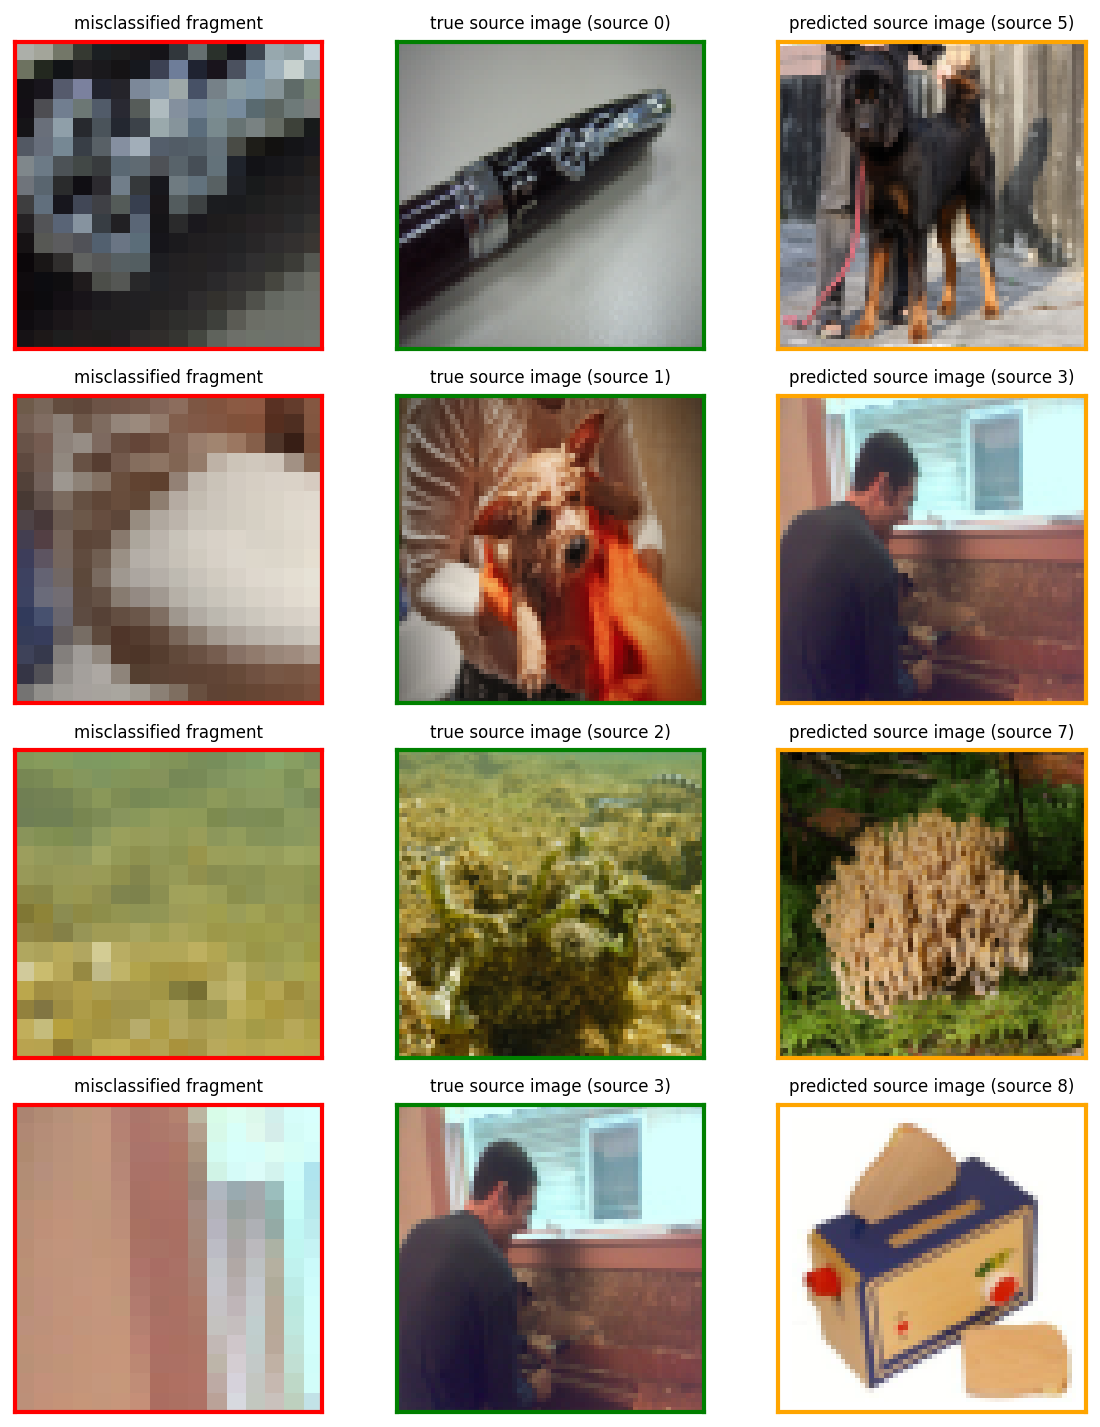
\includegraphics[width=0.85\textwidth]{failure_modes.png}
\caption{Failure modes from the current best checkpoint (\texttt{multitask_10}, best ARI = 0.570, $\beta = 0.01923$, $\lambda_{\mathrm{adj}} = 1.0$, $\lambda_{\mathrm{same}} = 1.0$, plain BCE on both heads). On the validation batch shown, 51 of 160 fragments were assigned to the wrong cluster after Hungarian matching of predicted to true labels. Each row shows: the misclassified fragment (left, red), the true source image it came from (middle, green), and the source image the model assigned it to (right, orange). Failures are dominated by near-uniform low-information fragments where multiple source images share the same dominant colour or texture --- an intrinsic ambiguity that no model trained on these $16 \times 16$ patches can resolve.}
\label{fig:failure-modes}
\end{figure}


A reliable taxonomy of failure modes would require aggregating misclassified
fragments across many batches, which we leave as follow-up work.

% ─────────────────────────────────────────────
\section{Decision Points Summary}
% ─────────────────────────────────────────────

\begin{center}
\begin{tabular}{lll}
\toprule
\textbf{Decision} & \textbf{Choice} & \textbf{Alternatives} \\
\midrule
Training objective & Adjacency prediction (pretext task) & Contrastive loss \\
Architecture & Siamese CNN + MLP head & Single encoder \\
Embedding combination & Diff $+$ product $+$ both embeddings & Concatenation only \\
Loss function & Binary cross-entropy & Focal loss (for imbalance) \\
Class imbalance & Weighted loss or negative subsampling & None \\
Clustering algorithm & Balanced spectral clustering & Plain spectral, $k$-means \\
Number of clusters & $k = 10$ (known) & Discovered automatically \\
Cluster size & Enforced ($G^2 = 16$) via Hungarian & Free \\
Eval batches per step & 20 (averaged) & 1 (single batch) \\
Evaluation metric & ARI, NMI & Purity \\
\bottomrule
\end{tabular}
\end{center}

% ─────────────────────────────────────────────
\section{Limitations}
% ─────────────────────────────────────────────

\begin{itemize}
    \item Adjacency is a local signal — it says nothing directly about fragments that are
          far apart within the same image. The model must generalise from local adjacency
          to global source identity.
    \item The graph has 12,720 edges. For larger grids or larger samples this grows
          quadratically and may become a bottleneck.
    \item The pretext metric and the task metric are misaligned. We train binary
          adjacency (only $\sim$1.9\% positives) but evaluate clustering. The model can
          achieve a useful similarity matrix (ARI $\approx 0.78$) while only mediocre
          on adjacency F1 ($\approx 0.26$), because adjacency is a sufficient but not
          necessary condition for same-source identity.
\end{itemize}

% ─────────────────────────────────────────────
\section{Further Suggestions}
% ─────────────────────────────────────────────

\paragraph{Differentiable surrogate for ARI.}
The training loss is on adjacency (or same-image), not on the downstream clustering
objective. A more direct alternative is to optimise a differentiable approximation of
ARI: the eigendecomposition and cluster-assignment steps of spectral clustering can be
relaxed via Sinkhorn iterations (as in SwAV) or via a MinCut-style differentiable graph
pooling. This would couple the representation learning to the clustering objective
explicitly. We did not pursue it because the multi-task same-image head already captures
most of the pairwise structure that ARI ultimately depends on, at a fraction of the
implementation cost.

\paragraph{Self-supervised pretrained encoder.}
DINOv2 \parencite{moco2020} or another self-supervised image encoder could replace our
trained-from-scratch CNN. Since these encoders use no labels, this stays within the
constraints of the task. Whether the gain (richer features) outweighs the loss
(features were trained at $224 \times 224$, not $16 \times 16$) is an open question.

\paragraph{Topology-aware clustering.}
The true partition is more constrained than ``equal sizes'': each cluster's induced
subgraph is isomorphic to a $G \times G$ grid (16 nodes, 24 edges, a planar graph with
maximum degree 4). A clustering algorithm that exploited this structure, e.g.\ a small
GNN trained to find equipartitions whose induced subgraphs are grid-like, could
disambiguate borderline assignments that pure spectral clustering misses. Implementation
cost is significant; the marginal benefit beyond what the model's already-strong soft
signal recovers is unclear.

\paragraph{Color-histogram baseline.}
A non-learned baseline using per-fragment color histograms with chi-square or EMD
distance, followed by spectral clustering, would anchor the learned model's ARI against
a meaningful reference. We expect this to be competitive on uniform-region fragments
and weak on textured ones; a controlled comparison would quantify how much of the 0.57
ARI comes from learned representation vs.\ trivial color matching.

\printbibliography

\end{document}
